\documentclass[landscape]{slides}

\addtolength\topmargin{-.4in}
\addtolength\textheight{.5in}

%%%%%%%%%%%%%%%%%%%%%%%%%%%%%%%%%%%%%%%%%%%%%%%%%%%%%%%%%%%%%%%%%%%%%%%%%%%%%%%
%
% TODO: 
%

%
% Note to self: color info - see grfguide.ps under shared tex directory
%
\usepackage{colordvi, pifont}
\usepackage[usenames,dvips]{color}
\usepackage{epsfig}

%
% Title and ornament defs blagged from eddie's hotnets talk
%
\def\ORN{{\large\Goldenrod{\Pisymbol{pzd}{106}}}}%
\def\T#1{\begin{center}\large\bfseries{\RoyalBlue{#1}}\par\vskip-40pt\ORN\end{center}}
\def\S#1{\begin{center}\large\bfseries{\RoyalBlue{#1}}\end{center}}
\begin{document}

\color{MidnightBlue}

%%%%%%%%%%%%%%%%%%%%%%%%%%%%%%%%%%%%%%%%%%%%%%%%%%%%%%%%%%%%%%%%%%%%%%%%%%%%%%%

\begin{slide}

\begin{center}

{\Large \textcolor{RoyalBlue}{RIP: Protocol Overview and Xorp Design}}

\ORN

\begin{tabular}{c}
\bf{Orion Hodson} \\
\MidnightBlue{International Computer Science Institute} \\
\end{tabular}

{\small August 2003}

\end{center}

\end{slide}

%%%%%%%%%%%%%%%%%%%%%%%%%%%%%%%%%%%%%%%%%%%%%%%%%%%%%%%%%%%%%%%%%%%%%%%%%%%%%%%

\begin{slide}

\T{Introducing the Routing Information Protocol}

\begin{dinglist}{228}

\item An Interior Gateway Protocol.

\item Based on distance vector \\
      (Ford and Fulkerson, Bellman-Ford).

% Use of DV goes back to origins of Internet - the ARPANET 1969.

\item Multiple variants on RIP (XNS, IPX, IP).

\item IP variants: RIPv1 (deprecated), RIPv2, and RIPng.

\end{dinglist}

\end{slide}

%%%%%%%%%%%%%%%%%%%%%%%%%%%%%%%%%%%%%%%%%%%%%%%%%%%%%%%%%%%%%%%%%%%%%%%%%%%%%%%

\begin{slide}

\T{Talk Outline}

\begin{dinglist}{228}

\item Distance Vector 101

\item RIP versions, docs, deltas

\item Proposed Xorp Design

\end{dinglist}

\end{slide}

%%%%%%%%%%%%%%%%%%%%%%%%%%%%%%%%%%%%%%%%%%%%%%%%%%%%%%%%%%%%%%%%%%%%%%%%%%%%%%%
%%
%% Distance Vector 101 section
%%

\begin{slide}

\T{Distance Vectors}

Nodes build and maintain a table of distances to other nodes and
exchange this with their peers.

Information received from peers is used to update table of distances
at receiving node.  Receiving only receives data from immediate peers
and knows their distance.

Updates are sent periodically.

Updates are \underline{SIMPLE} \ding{220} peer (or network) plus distance.

\end{slide}

%%%%%%%%%%%%%%%%%%%%%%%%%%%%%%%%%%%%%%%%%%%%%%%%%%%%%%%%%%%%%%%%%%%%%%%%%%%%%%%

\begin{slide}

\T{Classic Problem: Counting to Infinity}

\centering
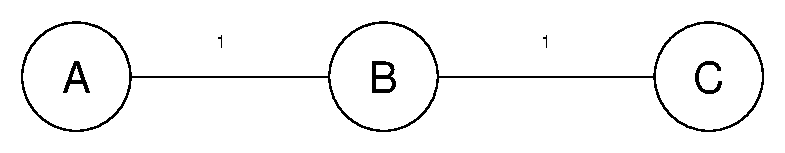
\epsfig{file=figs/3node.eps,width=0.5\textwidth}

\begin{tabular}{l|ccc}
Distance from C          & A & B & C \\
\ding{202} Stable point  & 2 & 1 & 0 \\
\ding{203} Link BC fails & 2 & ?? &  \\
\ding{204} A sends update (C at distance 2) & 2 & 3 \\
\ding{205} B sends update (C at distance 3) & 4 & 3 \\
\ding{206} A sends update (C at distance 4) & 4 & 5 \\
\ding{207} \ldots ad infinitum \ldots & \ldots & \ldots \\
\end{tabular}

\ding{220} Pick a small distance and call it infinity.

\end{slide}

%%%%%%%%%%%%%%%%%%%%%%%%%%%%%%%%%%%%%%%%%%%%%%%%%%%%%%%%%%%%%%%%%%%%%%%%%%%%%%%

\begin{slide}
\T{Hold-down}

\begin{center}
\framebox{
  \parbox{0.8\textwidth}{
    \centering
    In case of path failure, advertise
    path as infinity, and wait for ``hold-down'' interval.
  }
}
\end{center}

Okay, iff information reaches all nodes before hold-down timer
expires.

May slow convergence and does not solve count to infinity.

\end{slide}

%%%%%%%%%%%%%%%%%%%%%%%%%%%%%%%%%%%%%%%%%%%%%%%%%%%%%%%%%%%%%%%%%%%%%%%%%%%%%%%

\begin{slide}

\T{Split Horizons}

\begin{center}
\begin{tabular}{l|l}
\parbox{0.35\textwidth}{\bf Split Horizon} &
\parbox{0.35\textwidth}{\bf Split Horizon with } \\
 & {\bf Poison Reverse} \\

Don't advertise information & Advertise information \\
back to its source          & back to source with \\
                            & cost of infinity \\
\end{tabular}

\parbox{0.9\textwidth}{
Speeds up convergence in some cases (eg, A--B--C).

Solves some, but not all counting to infinity problems.
}

\end{center}

\end{slide}

%%%%%%%%%%%%%%%%%%%%%%%%%%%%%%%%%%%%%%%%%%%%%%%%%%%%%%%%%%%%%%%%%%%%%%%%%%%%%%%

\begin{slide}

\T{Counting to Infinity with a Split Horizon}

\begin{center}
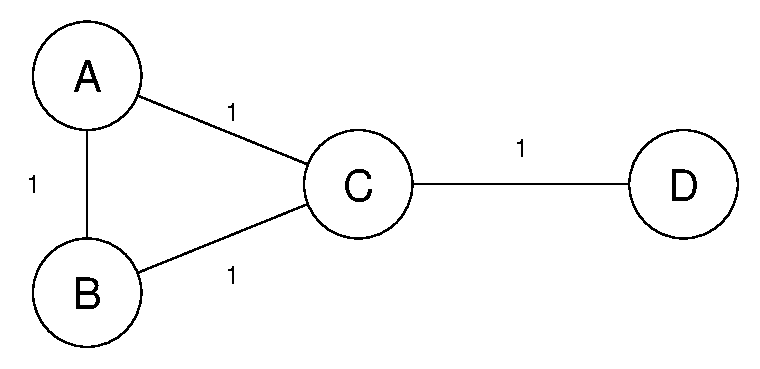
\epsfig{file=figs/split-horizon-1.eps,width=0.4\textwidth}

\begin{tabular}{l|cccc}
Distance from D                           & A & B & C & D \\
\ding{202} Stable point                  & 2 & 2 & 1 & 0 \\
\ding{203} Link CD fails \\
\ding{204} C believes D unreachable (SH) & 2 & 2 & \Pisymbol{psy}{165}\\
\ding{205} C sends update to A and B \\
\ding{206} C's update reaches B        & 2 & \Pisymbol{psy}{165} & \Pisymbol{psy}{165}\\
\ding{207} A sends periodic update       & 2 & 3 & \Pisymbol{psy}{165} \\
\ding{208} C's update reaches A          & \Pisymbol{psy}{165} & 3 & \Pisymbol{psy}{165}\\
\ding{209} B sends periodic update & \Pisymbol{psy}{165} & 3 & 4\\
\end{tabular}
\end{center}

\end{slide}

%%%%%%%%%%%%%%%%%%%%%%%%%%%%%%%%%%%%%%%%%%%%%%%%%%%%%%%%%%%%%%%%%%%%%%%%%%%%%%%

\begin{slide}

\T{Triggered Updates}

Fast propagation of changes (particularly for deleted nodes/links).

\begin{dinglist}{228}
\item Speeds convergence.
\end{dinglist}

\end{slide}

%%%%%%%%%%%%%%%%%%%%%%%%%%%%%%%%%%%%%%%%%%%%%%%%%%%%%%%%%%%%%%%%%%%%%%%%%%%%%%%
%%
%% RIP protocols, specs, features
%%

\begin{slide}
\T{RIP as a Distance Vector Protocol}
\begin{dinglist}{228}
\item Infinity fixed at 16.
\item Hold-down mandatory.
\item Split Horizon and Poison Reverse are recommended options.
\item Triggered updates mandatory for deleted routes, optional for new or changed routes.
\end{dinglist}

\end{slide}

%%%%%%%%%%%%%%%%%%%%%%%%%%%%%%%%%%%%%%%%%%%%%%%%%%%%%%%%%%%%%%%%%%%%%%%%%%%%%%%

\begin{slide}

\T{RIP: Some practicalities}

\begin{dinglist}{228}
\item Timers to age and timeout routes.
\item 2 Packet Types:  Request and Response.
\item Timer randomization.
\item Optional use of authentication.
\end{dinglist}

\end{slide}

%%%%%%%%%%%%%%%%%%%%%%%%%%%%%%%%%%%%%%%%%%%%%%%%%%%%%%%%%%%%%%%%%%%%%%%%%%%%%%%

\begin{slide}
\T{RIP Default Timer Values}

\begin{center}
\begin{tabular}{lc}
Timer & Period (s) \\ \hline
Route Expiry & 180 \\
Route Garbage Collection (hold-down) & 120\\
Periodic Updates & 25--35 \\
Triggered Update & 1--5 \\ \hline
\end{tabular}
\end{center}

\end{slide}

%%%%%%%%%%%%%%%%%%%%%%%%%%%%%%%%%%%%%%%%%%%%%%%%%%%%%%%%%%%%%%%%%%%%%%%%%%%%%%%

\begin{slide}
\T{RIP Request Messages}

Two variants:

{\bf Whole Table}\\
Used at start-up and response employs split horizon processing

{\bf Specific Routes}\\ 
Used for debugging and response does not employ split horizon\\

\end{slide}

%%%%%%%%%%%%%%%%%%%%%%%%%%%%%%%%%%%%%%%%%%%%%%%%%%%%%%%%%%%%%%%%%%%%%%%%%%%%%%%

\begin{slide}
\T{RIP Response Messages}

{\bf Query Response} \\
Response to a specific query

{\bf Regular update} \\
Contains all routes

{\bf Triggered update} \\
Contains route updates since last update (regular or triggered)

\centering
{\em Triggered updates are blocked by regular updates.}

\end{slide}

%%%%%%%%%%%%%%%%%%%%%%%%%%%%%%%%%%%%%%%%%%%%%%%%%%%%%%%%%%%%%%%%%%%%%%%%%%%%%%%

\begin{slide}

\T{Multi-Packet RIP Response Messages}

Packets hold finite number of route entries (25 for RIP on IPv4).  A
Response message will typically be composed of multiple packets.

Most vendors send trains of response messages with some small
inter-packet spacing to avoid buffer overflow.  10--50ms is typical.

\end{slide}

%%%%%%%%%%%%%%%%%%%%%%%%%%%%%%%%%%%%%%%%%%%%%%%%%%%%%%%%%%%%%%%%%%%%%%%%%%%%%%%

\begin{slide}
\T{RIP Response Message Route Entry Fields}

\begin{center}
\begin{tabular}{ll}
					  & {\bf Address} \\
Expected distance vector protocol fields: & {\bf Netmask} \\
					  & {\bf Cost}	  \\
\end{tabular}
\end{center}
Plus

{\bf Tag}\\ Protocol originating route if non-RIP, eg route redistribution.

{\bf Nexthop}\\
Used iff multiple routers exist on a LAN and nexthop is on LAN.  Avoids
unneeded hops.

\end{slide}

%%%%%%%%%%%%%%%%%%%%%%%%%%%%%%%%%%%%%%%%%%%%%%%%%%%%%%%%%%%%%%%%%%%%%%%%%%%%%%%

\begin{slide}
\T{RIP docs}

\begin{center}
\begin{tabular}{ll}
{\bf RFC} & {\bf Contents} \\ \hline
2453 & RIP version 2 \\
2080 & RIPng for IPv6 \\
1721 & RIP version 2: Protocol Analysis \\
1722 & RIP version 2: Applicability statement \\
1723 & RIP version 2: Carrying additional Info \\
1724 & RIP version 2: MIB Extension \\
2082 & RIP version 2: MD5 Authentication \\ \hline
\end{tabular}
\end{center}

\end{slide}

%%%%%%%%%%%%%%%%%%%%%%%%%%%%%%%%%%%%%%%%%%%%%%%%%%%%%%%%%%%%%%%%%%%%%%%%%%%%%%%

\begin{slide}
\T{RIP Protocols}

RIP v1: Class based, designed with expansion in mind.  UDP transport.
Fixed maximum packet size.

RIP v2: Extension of RIP v1. Classless. Supports tagged routes, next
hops, authentication.  Implementations typically interoperate with
RIPv1.

% RIPv1 inter-op is likely to be ugly.
% Authentication is none to pretty.

RIPng: As RIPv2, but relies on IPv6 for authentication mechanisms and
v1 equivalent interop.  Must have link-local addresses in packets as
source addresses and nexthops must have link-local addresses.  May use
path MTU discovery for packet sizes.

% The promised land :-)

\end{slide}

\begin{slide}

\T{Link-Local Addresses for RIPng}

Response packets must have a link-local source address.  This lessens
risk of accepting a packets from a router not on the link.
Additionally, the IP hop count field is set to 255 to strengthen this
condition.

When nexthops are present in response packets, they are specified as
link-local addresses.  By definition, nexthops are only specified only
links where the nexthop router is visible on the link - the goal being
to avoid bouncing traffic between multiple routers that are on the
link.

\end{slide}

%%%%%%%%%%%%%%%%%%%%%%%%%%%%%%%%%%%%%%%%%%%%%%%%%%%%%%%%%%%%%%%%%%%%%%%%%%%%%%%
%%
%% Design notes
%%

\begin{slide}

\T{First Cut Features}

Functional RIPv2 and RIPng implementation\\
Highly similar \ding{220} templates with limited specialization

Scale to O(10000) \ding{220} small state including a timer per route

Support tunable timer abd packet spacing values

SNMP support

\end{slide}

%%%%%%%%%%%%%%%%%%%%%%%%%%%%%%%%%%%%%%%%%%%%%%%%%%%%%%%%%%%%%%%%%%%%%%%%%%%%%%%

\begin{slide}

\T{Later Work}

Tagged route filtering to help manage route redistribution.

RIPv1 and RIPv1 Inter-Op.

\end{slide}

%%%%%%%%%%%%%%%%%%%%%%%%%%%%%%%%%%%%%%%%%%%%%%%%%%%%%%%%%%%%%%%%%%%%%%%%%%%%%%%

\begin{slide}

\T{RIP Interaction with Xorp processes}
\centering

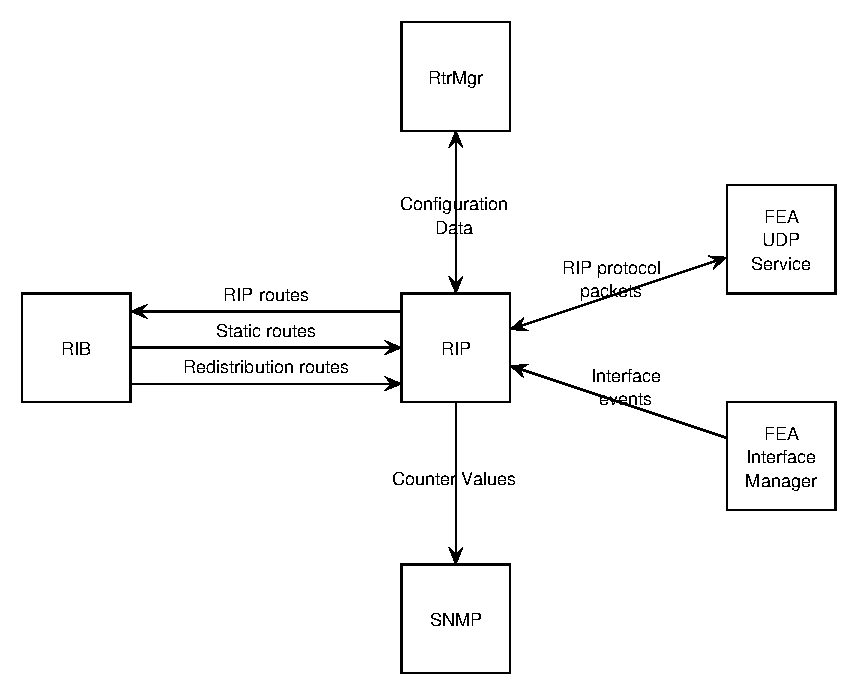
\epsfig{file=figs/rip-processes-interaction.eps,width=0.7\textwidth}

\end{slide}

%%%%%%%%%%%%%%%%%%%%%%%%%%%%%%%%%%%%%%%%%%%%%%%%%%%%%%%%%%%%%%%%%%%%%%%%%%%%%%%

\begin{slide}

\T{At the core: Peers, Routes, RouteDatabase}

\centering
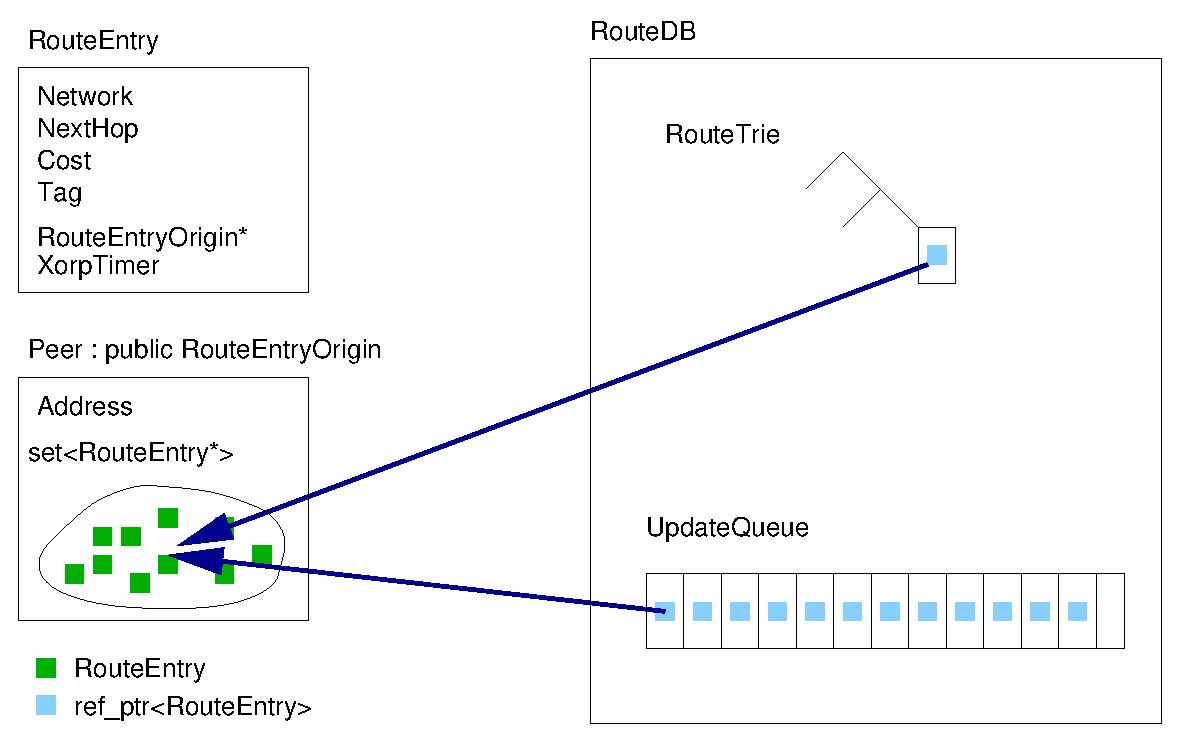
\epsfig{file=figs/core.eps,width=0.8\textwidth}

\end{slide}

%%%%%%%%%%%%%%%%%%%%%%%%%%%%%%%%%%%%%%%%%%%%%%%%%%%%%%%%%%%%%%%%%%%%%%%%%%%%%%%

\begin{slide}

\T{Route Management}

{\tt RouteEntryOrigin} objects own {\tt RouteEntry} objects.  {\tt RouteEntry} objects
associate and dissociate themselves from {\tt RouteEntryOrigin} on
construction and destruction.

{\tt RouteDB} is shared {\tt RouteEntry} store - contains
{\tt RouteDB::RouteTrie} and {\tt UpdateQueue}.

{\tt RouteDB::RouteTrie} is used for lookup and modify operations.  {\tt RouteEntryOrigin}
objects may be used for table ``dump'' operations (much faster).

{\tt UpdateQueue} is used for triggered updates and is a vector
reference counted {\tt RouteEntry} objects.  Route can be removed from Trie,
and just exist in the may exist in {\tt UpdateQueue}.

\end{slide}

%%%%%%%%%%%%%%%%%%%%%%%%%%%%%%%%%%%%%%%%%%%%%%%%%%%%%%%%%%%%%%%%%%%%%%%%%%%%%%%

\begin{slide}

\T{Core Classes and their Relationships}

\centering
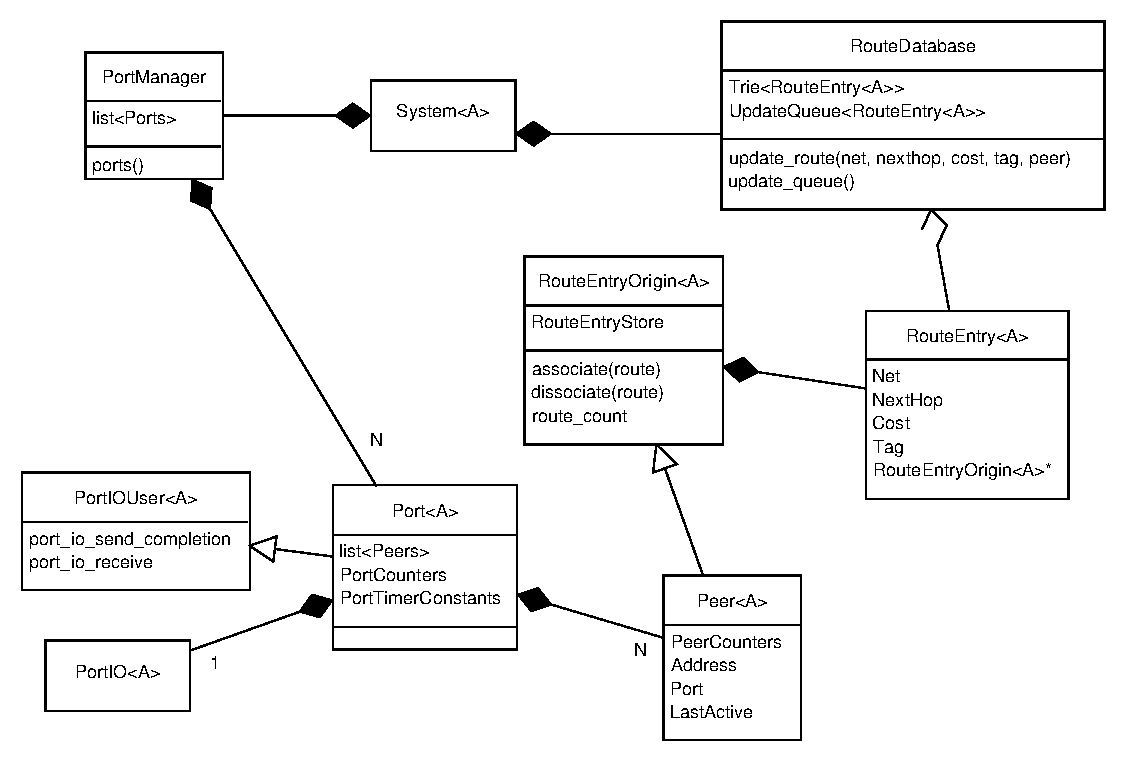
\epsfig{file=figs/rip-10000.eps,width=0.8\textwidth}

\end{slide}

%%%%%%%%%%%%%%%%%%%%%%%%%%%%%%%%%%%%%%%%%%%%%%%%%%%%%%%%%%%%%%%%%%%%%%%%%%%%%%%

\begin{slide}

\T{Port Objects}

A {\tt Port} potentially exists for each Xorp VIF and bound to an
address on a VIF.

{\tt Port} objects manage $0...N$ {\tt Peer} objects.

{\tt Port} objects are instantiated by {\tt PortFactory} instances and
managed by the {\tt PortManager} object.

\end{slide}

%%%%%%%%%%%%%%%%%%%%%%%%%%%%%%%%%%%%%%%%%%%%%%%%%%%%%%%%%%%%%%%%%%%%%%%%%%%%%%%

\begin{slide}

\T{Port Objects: Input and Output Processing}

\begin{dinglist}{228}
\item Receives request and response messages from {\tt PortIO<A>}.
\item Performs authentication.
\item Feeds routes and updates into {\tt Peer object} and {\tt RouteDB
  objects} (with optional Split Horizon/Poison Reverse).
\item Holds a read iterator to {\tt UpdateQueue} and has a timer for
  triggered updates (walk read iterator to end of {\tt UpdateQueue}).
\end{dinglist}
\end{slide}


%%%%%%%%%%%%%%%%%%%%%%%%%%%%%%%%%%%%%%%%%%%%%%%%%%%%%%%%%%%%%%%%%%%%%%%%%%%%%%%

\begin{slide}
\T{Periodic updates}

Periodic updates involve sending the entire contents of the RIP route
database.  Typically every 30 +/- 5s.

Two options:
\begin{dinglist}{106}
\item Perform periodic updates by trawling routes and handling all {\tt
Port} instances simultaneously.  (Less work, correlated output).
\item Perform periodic updates on a per {\tt Port} instance basis.
(More work, decorrelated output). [Preferred]
\end{dinglist}

\end{slide}

%%%%%%%%%%%%%%%%%%%%%%%%%%%%%%%%%%%%%%%%%%%%%%%%%%%%%%%%%%%%%%%%%%%%%%%%%%%%%%%

\begin{slide}
\T{Per Peer Periodic Update [Proposed]}

Each peer has a {\tt PeriodicUpdater} class that iterates through list
of peers and their sets of routes each time a periodic update is
required.  The {\tt PeriodicUpdater} is timer driven and outputs 1
response packet per each time it's scheduled.  The timer expiry
interval is set to the interpacket spacing and the {\tt
PeriodicUpdater} run until it has output all the routes.

The {\tt PeriodicUpdater} maintains a reference to the last route it
puts in each response packet so iteration through a {\tt Peer} objects
set of {\tt RouteEntry} objects can always resume from a valid 
{\tt RouteEntry}.

\end{slide}

%%%%%%%%%%%%%%%%%%%%%%%%%%%%%%%%%%%%%%%%%%%%%%%%%%%%%%%%%%%%%%%%%%%%%%%%%%%%%%%

\begin{slide}
\T{RIB Interaction}

{\bf Input}\\
{\tt RIBPeer} class for storing routes learned from RIB.
No Timers on these routes in {\tt RouteDB}.

{\bf Output}\\
{\tt RIBOutput} class that is attached as a read-iterator to {\tt UpdateQueue}.

{\bf DebugOutput} [option]\\
{\tt AnyTargetOutput} as RIBOutput, but more generic.
\end{slide}

%%%%%%%%%%%%%%%%%%%%%%%%%%%%%%%%%%%%%%%%%%%%%%%%%%%%%%%%%%%%%%%%%%%%%%%%%%%%%%%

\begin{slide}

\T{XRL Interfaces}

Separate XrlTargets for IPv4 and IPv6 RIP systems.

Interface details to be decided.

All objects reachable from Top-Level {\tt System} object.

SNMP counters are (mostly) in place.

\end{slide}

%%%%%%%%%%%%%%%%%%%%%%%%%%%%%%%%%%%%%%%%%%%%%%%%%%%%%%%%%%%%%%%%%%%%%%%%%%%%%%%

\end{document}

